\documentclass[tikz]{standalone}
\usepackage{tikz}
\usepackage[AutoFakeBold=true,AutoFakeSlant=true]{xeCJK}
\usepackage[zihao=-4,UTF8,heading=true]{ctex}
\usepackage[simplified]{pgf-umlcd}
\usetikzlibrary{fit} %形状
\usetikzlibrary{positioning} %不加方向运算可能出错
\usetikzlibrary{arrows.meta} %箭头
\usetikzlibrary{calc}

\setCJKmainfont{微软雅黑}
\begin{document}
	\thispagestyle{empty}
    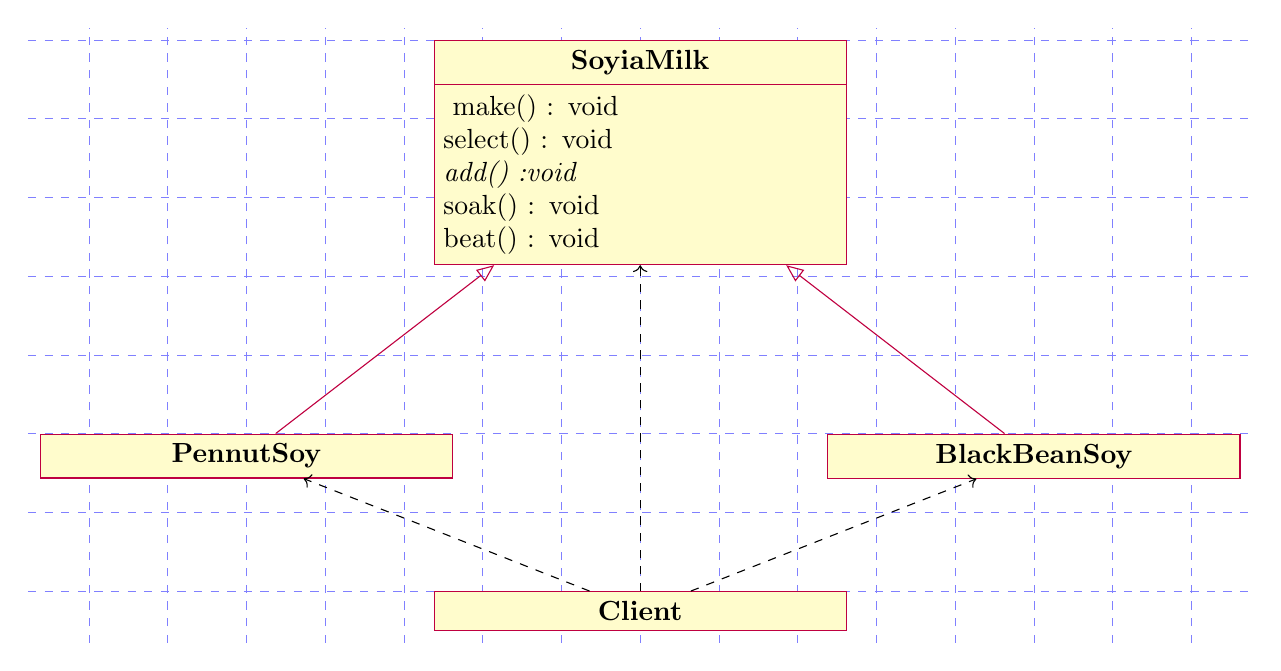
\begin{tikzpicture}[show background grid]
        \begin{class}[text width=5cm]{SoyiaMilk}{0,0}
            \operation{ make() : void}
            \operation{ select() : void}
            \operation[0]{ add() :void }
            \operation{ soak() : void}
            \operation{ beat() : void}
        \end{class}
        \begin{class}[]{BlackBeanSoy}{5,-5}
            \inherit{SoyiaMilk}
        \end{class}
        \begin{class}[]{PennutSoy}{-5,-5}
            \inherit{SoyiaMilk}
        \end{class}
        \begin{class}[]{Client}{0,-7}
        \end{class}
        \draw [dashed, ->] (Client) -- (SoyiaMilk);
        \draw [dashed, ->] (Client) -- (PennutSoy);
        \draw [dashed, ->] (Client) -- (BlackBeanSoy);

    \end{tikzpicture}

\end{document}